\documentclass[]{scrartcl}

%\usepackage{fullpage}
\usepackage{graphicx}
\usepackage[T1]{fontenc}

\usepackage[unicode=true,pdfusetitle,
bookmarks=true,bookmarksnumbered=false,bookmarksopen=false,
breaklinks=true,pdfborder={0 0 0},pdfborderstyle={},backref=false,colorlinks=true]
{hyperref}
\hypersetup{linkcolor=blue,citecolor=blue,urlcolor=blue}
\usepackage[backend=biber, maxbibnames=99, style=numeric]{biblatex}
\setlength\bibitemsep{2\itemsep}
\addbibresource{refs.bib}

%opening
\title{Report to the Guam Invasive Species Council on University of Guam Invasive Species Activities}
\author{Aubrey Moore}

\begin{document}

\maketitle

\section{Pacific Ecological Security Conference (PESC)}

The PESC, held in Palau during October 2022, brought together island leaders, development partners, regional organizations, agricultural/food security and natural resource managers, and the media to discuss the importance of managing and preventing the spread of invasive species in Pacific Island environments \cite{anonymousFirstPacificEcological2022}.

 Conference hosts and sponsors included Government of Palau Ministry of Agriculture, Fisheries, and Environment, Secretariat of the Pacific Community (SPC), the East-West Center, the Global Environment Facility (GEF), the Nature Conservancy, the US Department of the Interior - Office of Insular Affairs, the U.S. Forest Service, and the Ocean Policy Research Institute.

Delegates from Guam were Roland Quitugua and Aubrey Moore from UOG and Glenn Dulla and Andrea Blas from the Department of Agriculture. The Guam delegation participated in a satellite meeting organized by the U.S. Department of the Interior - Office of Insular Affairs and the U.S. Forest Service. At this meeting each island group presented a status report on invasive species issue (See \parencite{mooreOverviewInvasiveSpecies2022-10-06} for slides from the Guam presentation). This was followed by discussions on federal funding and collaboration.  

\subsection{Strategic Action Plan for Coconut Rhinoceros Beetle (CRB)}

Prior to the PESC, members of the Guam delegation worked with colleagues throughout the Pacific to write a Pacific-wide strategic action plan for response to the recent spread of CRB. This plan was accepted by PESC delegates and has been published online \cite{conferenceStrategicActionPlan2022}.

\newpage

The plan includes five objectives:

\begin{enumerate}
	\item Enhance Regional Coordination and support of PICTs to achieve the
	objectives of the CRB Strategic Action Plan (SAP)
	\item Conduct immediate and long-term collaborative research to develop
	tools and understanding necessary to enable effective CRB prevention, control, and
	eradication
	\item Prevent the spread of CRB to new locations in the Pacific region and
	beyond
	\item Implement an active early detection, and rapid response system for new
	outbreaks at regional and island levels
	\item Improve implementation of control efforts and mitigate the impacts of
	CRB where already present in the region
	
\end{enumerate} 

\section{Recently Detected Invasive Species}

\subsection{Citrus blackfly, \textit{Aleurocanthus woglumi}}

This major pest of citrus was first detected on Guam in March 2023 \cite{moore2023}. It is not expected to cause major damage because it is parasitized by biological control agents introduced for a closely related insect pest, the orange spiny whitefly, \textit{A. spiniferus}.

\section{Work on Coconut Rhinoceros Beetle (CRB)}

\subsection{Island-wide CRB Damage Survey}

\cite{moorePressRelease2023}

% TODO: \usepackage{graphicx} required
\begin{figure}[h]
	\centering
	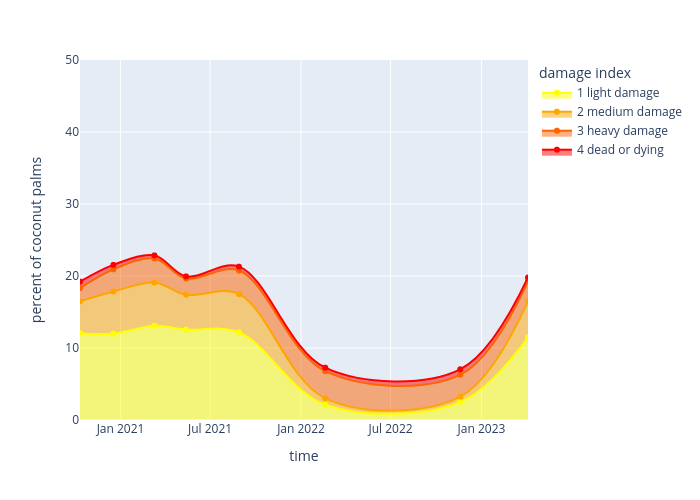
\includegraphics[width=0.7\linewidth]{images/timeline}
	\caption{caption here}
	\label{fig:timeline}
\end{figure}


\subsection{CRB Biological Control}

\section{Work on Cycad Aulacaspis Scale (CAS)}

\newpage
\printbibliography

\end{document}
